% -*- Mode:TeX -*-


\documentclass[11pt,twoside,singlespace]{report}
%\pagestyle{plain}
%\pagestyle{headings}
%\lhead{\chaptermark}

\usepackage{amssymb,amsmath} % better maths commands
\usepackage{graphicx}
\usepackage{verbatim}  % allows 'comment' environment, which is useful for commenting out multi-line sections
%\usepackage{txfontsb}
\usepackage{mymanual}
\graphicspath{{graphics/}}
\usepackage[usenames]{color}
%\maxtocdepth{section}
\usepackage[sort&compress,numbers]{natbib} % better citations
\usepackage{fancyhdr}
%\usepackage[nottoc,notlot,notlof]{tocbibind}
\usepackage{url}
\usepackage{hyperref}
\hypersetup{colorlinks=true,linkcolor=blue}

\newcommand{\vv}{\upsilon}
\newcommand{\vect}[1]{{\mathbf #1}}
\newcommand{\regcoil}{{\ttfamily regcoil}}
\newcommand{\regcoilPlot}{{\ttfamily regcoilPlot}}
\newcommand{\netCDF}{{\ttfamily netCDF}}
\newcommand{\fortran}{{\ttfamily fortran}}
\newcommand{\matlab}{{\ttfamily matlab}}
\newcommand{\python}{{\ttfamily python}}
\newcommand{\nescoil}{{\ttfamily nescoil}}
\newcommand{\bnorm}{{\ttfamily bnorm}}
\newcommand{\nfp}{{\ttfamily nfp}}
\newcommand{\parlink}[1]{{\ttfamily \hyperlink{#1}{#1}}}
\newcommand{\vmec}{{\ttfamily vmec}}
\newcommand{\todo}[1]{\textcolor{red}{To do: #1}}

\graphicspath{{figures/}}

% uncomment the following line to remove all graphics (for faster compiling)
%\renewcommand{\includegraphics}[2][x]{}

\newcommand{\boldkappa}{{\mathbf \kappa}}

\setlength{\oddsidemargin}{0.25in}	% 1.25in left margin
\setlength{\evensidemargin}{0.25in}	% 1.25in left margin (even pages)
\setlength{\topmargin}{0.0in}		% 1in top margin
\setlength{\textwidth}{6.0in}		% 6.0in text - 1.25in rt margin
\setlength{\textheight}{8.6in}		% Body ht for 1in margins

\setcounter{tocdepth}{1}
\begin{document}


\begin{center}

\vspace*{1in}

{\Huge QUASISYMMETRY User Manual}

\vspace{2in}

\centerline{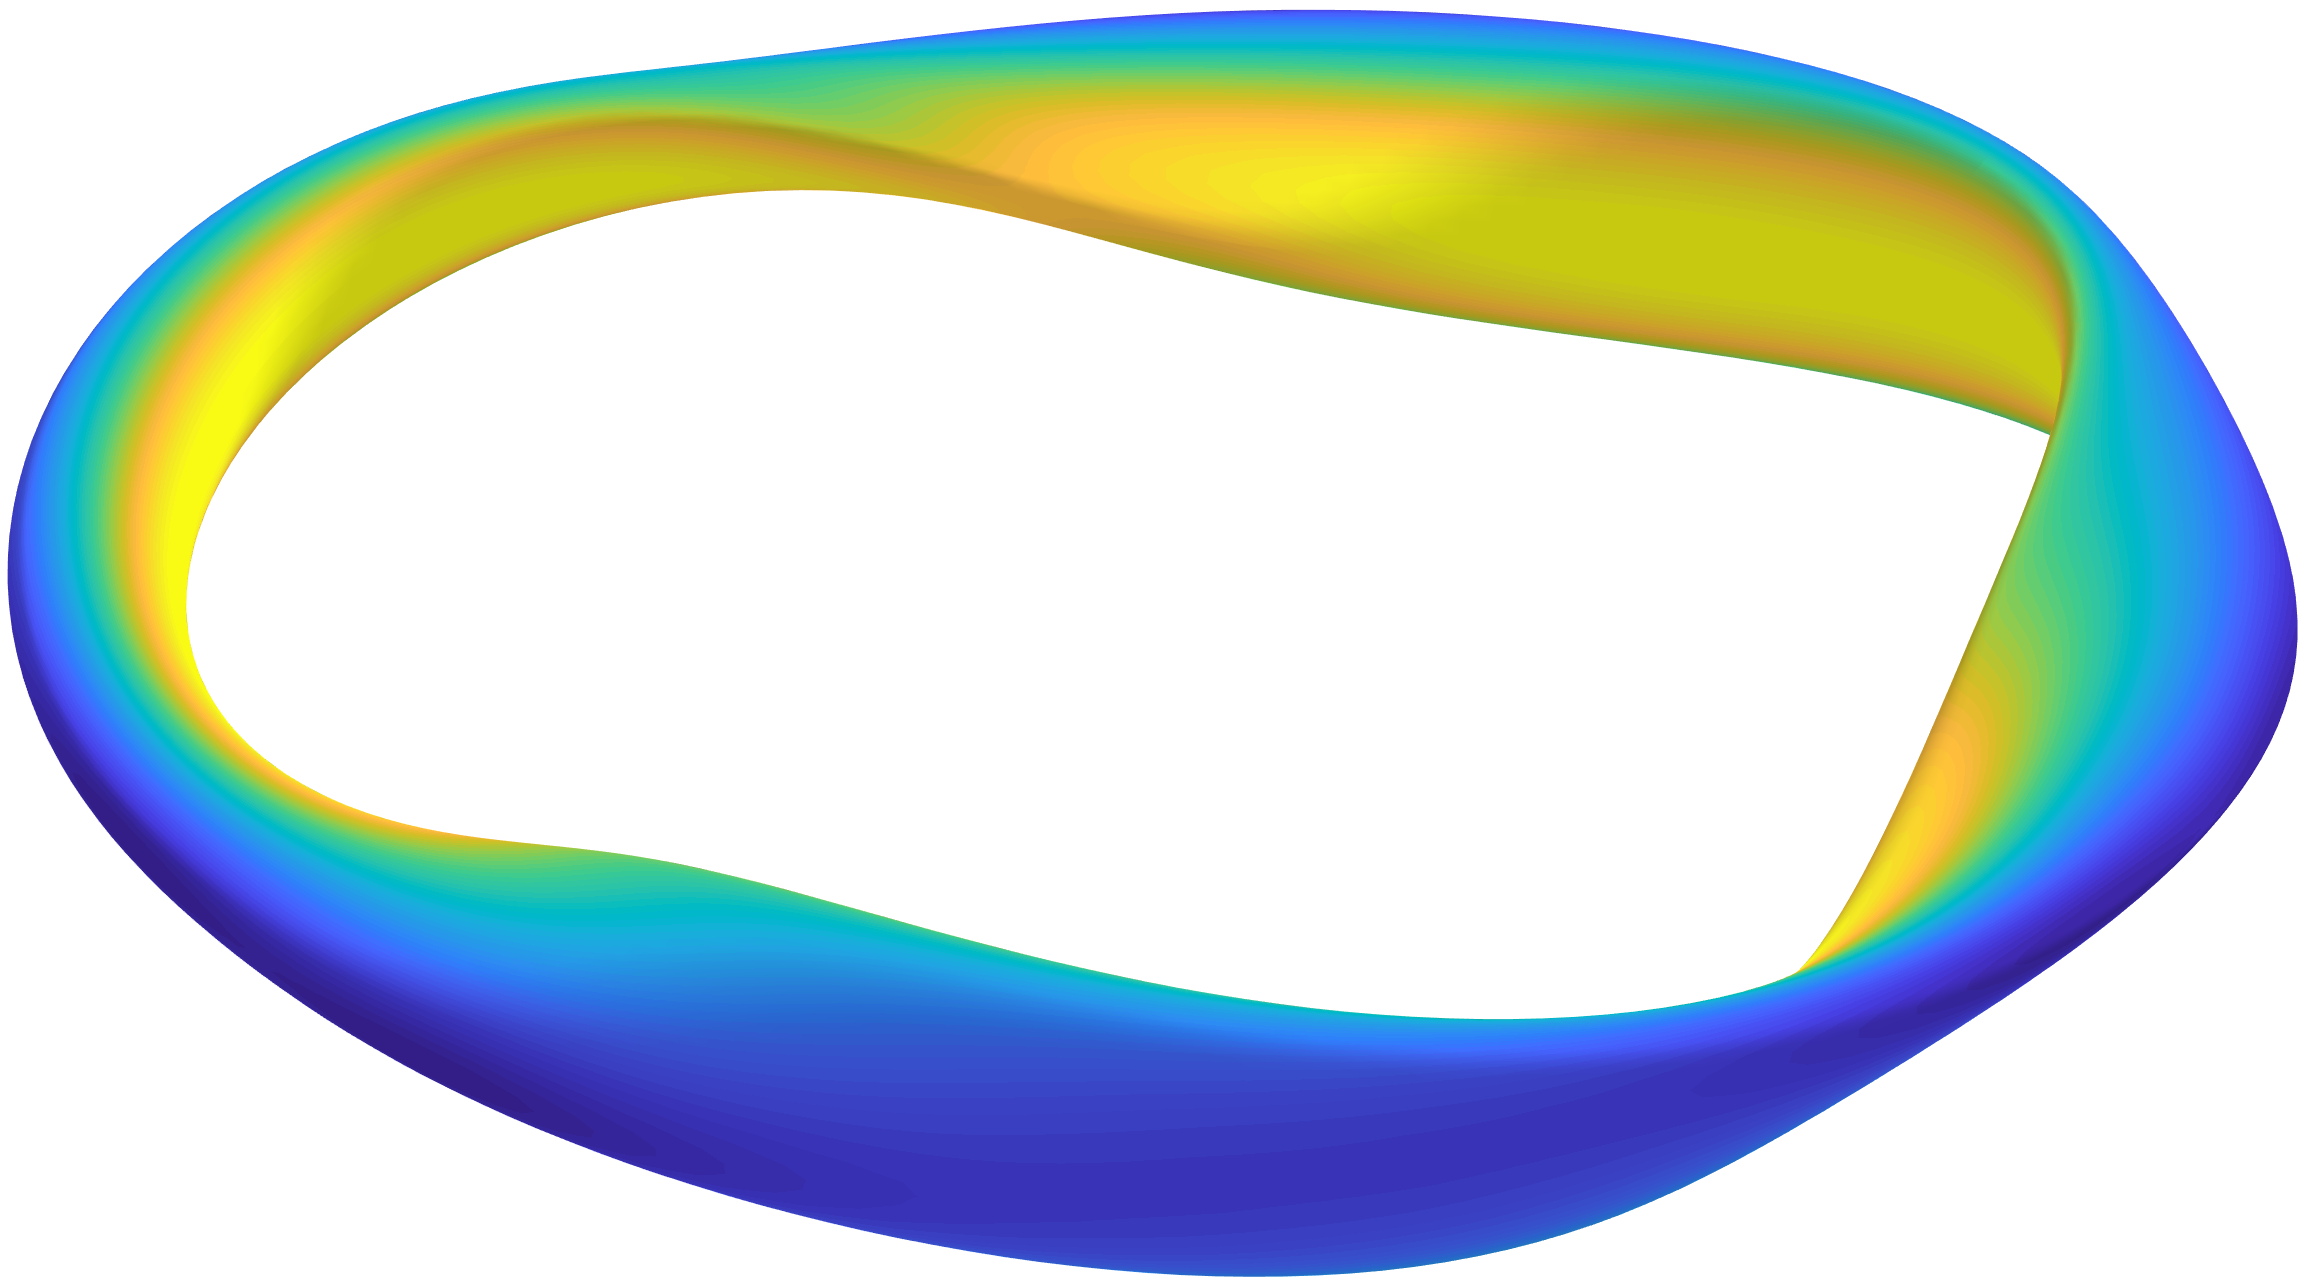
\includegraphics[width=6.5in]{m20180404_02_plotQuasisymmetricSolutionForPaperII_a.png}}

%{\Large Version 3}

\vspace{1.0in}

Revised January 26, 2017

\end{center}




%\pagestyle{plain}
\fancyhf{}
\cfoot{\thepage}
\tableofcontents

\clearpage


\pagestyle{fancy}
\fancyhf{}
\lhead[\thepage]{\leftmark}
\rhead[\leftmark]{\thepage}
%\lhead{\chaptermark}
\renewcommand{\chaptermark}[1]{\markboth{\sc{\chaptername\ \thechapter.\ #1}}{}}
\setlength{\headsep}{6pt}

\setlength{\parskip}{0pt plus 0pt minus 0pt}

% Main chapters go here:
\chapter{Overview}

This program constructs the shapes of stellarators that are quasisymmetric to first
order in the distance from the magnetic axis.
The method is based on the theory in \cite{GB1,GB2}
and the numerical method in \cite{PaperII}.
This latter paper is available in the Git repository for this program.



\section{Required libraries}

\begin{itemize}

\item {\ttfamily LAPACK} (for solving linear systems)
\item {\ttfamily MPI} (for parallelization of parameter scans)
\item {\ttfamily NetCDF} (for writing the output file)

\end{itemize}

Most of these libraries will be available on any high-performace computing system. {\ttfamily LAPACK}
is available on Apple Mac computers (as part of the Accelerate framework) if you install Xcode through the App store.

The {\ttfamily make test} scripts use \python~(version 2.7),
{\ttfamily numpy}, and {\ttfamily scipy}.
The plotting scripts {\ttfamily quasisymmetryPlotSingle}, {\ttfamily quasisymmetryPlotCompare}, and {\ttfamily quasisymmetryPlotScan} uses the same \python~libraries
as well as {\ttfamily matplotlib}.

\section{Cloning the repository}

The source code for \quasisymmetry~is hosted in a {\ttfamily git} repository at
\url{https://github.com/landreman/quasisymmetry}.
You obtain the \quasisymmetry~source code by cloning the repository. This requires several steps.

\begin{enumerate}
\item Create an account on \url{github.com}, and sign in to {\ttfamily github}.
\item Click the icon on the top right to see the drop-down menu of account options, and select the ``Settings'' page.
\item Click on ``SSH and GPG keys'' on the left, and add an SSH key for the computer you wish to use. To do this, you may wish to read see the ``generating SSH keys'' guide which is linked to from that page: \url{https://help.github.com/articles/connecting-to-github-with-ssh/}
\item From a terminal command line in the computer you wish to use, enter\\
{\ttfamily git clone git@github.com:landreman/quasisymmetry.git}\\
 to download the repository.
\end{enumerate}

Any time after you have cloned the repository in this way, you can download future updates to the code by entering {\ttfamily git pull} from any subdirectory within your local copy.



\section{Single calculations vs. scans}

The code has two basic modes of operation, {\ttfamily general\_option = "single"} vs {\ttfamily "scan"}. 
When {\ttfamily general\_option = "single"}, a single set of input parameters (magnetic axis shape etc) is
considered, and a VMEC input file is generated. When {\ttfamily general\_option = "scan"},
the input parameters are scanned, and no VMEC input file is generated. For either option, results
are saved in a NetCDF file. The variables that are saved in the NetCDF file are different depending on
{\ttfamily general\_option}.

\section{Parallelization}

When computing the shape of a single configuration, the calculation is so fast (typically on the order of 1 ms)
that parallelization is unnecessary. However parallelization is useful when doing parameter scans,
in which case the calculation is `embarassingly parallel'. MPI is used for this latter case.


\section{\ttfamily make test}

To test that your \quasisymmetry~executable is working, you can run {\ttfamily make test}.  Doing so will run
\quasisymmetry~for some or all of the examples in the {\ttfamily examples/} directories.
After each example completes, several of the output quantities
will be checked, using the
{\ttfamily tests.py} script in the example's directory.
The {\ttfamily make test} feature is very useful when making changes to the code, since it allows you to check
that your code modifications have not broken anything and that previous results
can be recovered.

If you run {\ttfamily make retest},
no new runs of \quasisymmetry~will be performed, but the {\ttfamily tests.py} script
will be run on any existing output files in the \path{/examples/} directories.

\section{Units}

As in \vmec, all of \quasisymmetry's input and output parameters use SI units: meters, Teslas, Amperes, and combinations thereof.

\section{Plotting results}

The python program \quasisymmetryPlotSingle~will display some of the results from a \quasisymmetry~calculation with {\ttfamily general\_option="single"}.
Multiple such runs can be compared on a single figure using the script {\ttfamily quasisymmetryPlotCompare}.
The python program \quasisymmetryPlotScan~will display some of the results from a \quasisymmetry~parameter scan.

\section{Output quantities}

The output variables are documented using metadata (the `{\ttfamily long\_name}' attribute)
in the netCDF output files {\ttfamily quasisymmetry\_out.<extension>.nc}.
To view the available output variables, their annotations, and their values, you can run
{\ttfamily ncdump quasisymmetry\_out.<extension>.nc | less} from the command line.
Some of the most commonly used output quantities which can be found in the netCDF file are 
{\ttfamily iotas},
{\ttfamily max\_curvatures},
{\ttfamily max\_elongations},
{\ttfamily axis\_helicities},
{\ttfamily scan\_R0c},
{\ttfamily scan\_Z0s},
and
{\ttfamily scan\_eta\_bar}.

\section{Questions, Bugs, and Feedback}

We welcome any contributions to the code or documentation.
For write permission to the repository, or to report any bugs, provide feedback, or ask questions, contact Matt Landreman at
\href{mailto:matt.landreman@gmail.com}{\nolinkurl{matt.landreman@gmail.com} }







\chapter{Input Parameters}
\label{ch:input}

\newcommand{\param}[5]{{\setlength{\parindent}{0cm} {\ttfamily \bfseries \hypertarget{#1}{#1}}\\{\it Type}: #2\\{\it Default}: #3\\{\it When it matters}: #4\\{\it Meaning}: #5}}
\newcommand{\myhrule}{{\setlength{\parindent}{0cm} \hrulefill }}

\newcommand{\true}{{\ttfamily .true.}}
\newcommand{\false}{{\ttfamily .false.}}

In this section we describe all the parameters which can be included in the input namelist. \\

%%%%%%%%%%%%%%%%%%%%%%%%%%%%%%%%%%%%%%%%%%%%%%%%%%%%%%%%%%%%%%%%%%%5
%%%%%%%%%%%%%%%%%%%%%%%%%%%%%%%%%%%%%%%%%%%%%%%%%%%%%%%%%%%%%%%%%%%5

\section{General parameters}

\param{general\_option}
{string}
{{\ttfamily "single"}}
{Always}
{Determines the overall flow of program execution.\\

{\ttfamily general\_option} = {\ttfamily "single"}: Solve the equations for first-order quasisymmetry for a single set of input parameters.\\

{\ttfamily general\_option} = {\ttfamily "scan"}: Solve the equations for first-order quasisymmetry for a range of input parameters.\\

}

\myhrule

\param{verbose\_option}
{string}
{{\ttfamily "all"}}
{Only when \parlink{general\_option}={\ttfamily "scan"}}
{Determines how much information is printed to the standard output during a scan.\\

{\ttfamily verbose\_option} = {\ttfamily "all"}: Full information is printed for all solves on all processors.\\

{\ttfamily verbose\_option} = {\ttfamily "proc0"}: Full information is printed for all solves on processor 0, while no information is printed by other processors.\\

{\ttfamily verbose\_option} = {\ttfamily "summary"}: Minimal information is printed.\\
}

\myhrule

\param{max\_elongation\_to\_keep}
{double}
{10}
{Only when \parlink{general\_option}={\ttfamily "scan"}}
{Only configurations with elongation equal to or below this value are saved in the output file.}

\myhrule

\param{vmec\_template\_filename}
{string}
{{\ttfamily ""}}
{Only when \parlink{general\_option}={\ttfamily "single"}}
{A fortran namelist file containing a vmec {\ttfamily \&indata} namelist. This namelist will be copied to create a new vmec input file based on the solution of the Garren-Boozer problem, except for the quantities that are overwritten: the axis shape, boundary shape, number of field periods, {\ttfamily nfp}, and {\ttfamily lasym}. Also {\ttfamily lfreeb} will be set to false.}

\myhrule

\param{r}
{double}
{0.1}
{Only when \parlink{general\_option}={\ttfamily "single"}}
{Effective minor radius that will be used in the new vmec input file.  This parameter is identical to $r$ in \cite{PaperII}. Note that this parameter does not enter the Garren-Boozer problem directly; it only affects the transformation to a finite-aspect-ratio result.}

\myhrule

%%%%%%%%%%%%%%%%%%%%%%%%%%%%%%%%%%%%%%%%%%%%%%%%%%%%%%%%%%%%%%%%%%%5
%%%%%%%%%%%%%%%%%%%%%%%%%%%%%%%%%%%%%%%%%%%%%%%%%%%%%%%%%%%%%%%%%%%5

\section{Specifying a single calculation}

\param{R0c}
{double array}
{[0,0,...]}
{Only when \parlink{general\_option}={\ttfamily "single"}}
{Fourier mode amplitudes of the magnetic axis shape. Elements of this array corresp\
ond to toroidal modes 0, \parlink{nfp}, 2$\times$\parlink{nfp}, 3$\times$\parlink{nfp}, etc.  The cylindrical coordinate $R$ is determined by
\begin{equation}
R(\phi) = \sum_{n=0}^{\infty} \left[ (\mathtt{R0c})_{n+1} \cos( (\mathtt{nfp})n\phi) +  (\mathtt{R0s})_{n+1} \sin( (\mathtt{nfp})n\phi)\right].
\label{eq:Rseries}
\end{equation}
Note that when \parlink{general\_option}={\ttfamily "scan"}, the code overwrites {\ttfamily R0c} with values between \parlink{R0c\_min} and \parlink{R0c\_max}.
}

\myhrule

\param{R0s}
{double array}
{[0,0,...]}
{Only when \parlink{general\_option}={\ttfamily "single"}}
{Fourier mode amplitudes of the magnetic axis shape. Elements of this array correspond to toroidal modes 0, \parlink{nfp}, 2$\times$\parlink{nfp}, 3$\times$\parlink{nfp}, etc. See (\ref{eq:Rseries}).
Note that when \parlink{general\_option}={\ttfamily "scan"}, the code overwrites {\ttfamily R0s} with values between \parlink{R0s\_min} and \parlink{R0s\_max}.
}

\myhrule

\param{Z0c}
{double array}
{[0,0,...]}
{Only when \parlink{general\_option}={\ttfamily "single"}}
{Fourier mode amplitudes of the magnetic axis shape. Elements of this array correspond to toroidal modes 0, \parlink{nfp}, 2$\times$\parlink{nfp}, 3$\times$\parlink{nfp}, etc. The cylindrical coordinate $Z$ is determined by
\begin{equation}
Z(\phi) = \sum_{n=0}^{\infty} \left[ (\mathtt{Z0c})_{n+1} \cos((\mathtt{nfp})n \phi) +  (\mathtt{Z0s})_{n+1} \sin((\mathtt{nfp})n \phi)\right].
\label{eq:Zseries}
\end{equation}
Note that when \parlink{general\_option}={\ttfamily "scan"}, the code overwrites {\ttfamily Z0c} with values between \parlink{Z0c\_min} and \parlink{Z0c\_max}.
}

\myhrule

\param{Z0s}
{double array}
{[0,0,...]}
{Only when \parlink{general\_option}={\ttfamily "single"}}
{Fourier mode amplitudes of the magnetic axis shape. Elements of this array correspond to toroidal modes 0, \parlink{nfp}, 2$\times$\parlink{nfp}, 3$\times$\parlink{nfp}, etc. See (\ref{eq:Zseries}).
Note that when \parlink{general\_option}={\ttfamily "scan"}, the code overwrites {\ttfamily Z0s} with values between \parlink{Z0s\_min} and \parlink{Z0s\_max}.
}

\myhrule

\param{eta\_bar}
{double}
{1.0}
{Only when \parlink{general\_option}={\ttfamily "single"}}
{Garren and Boozer's parameter $\bar{\eta}$. For a given axis shape, different values of this parameter result in different solutions for quasisymmetric flux surface shapes.
}

\myhrule

\param{sigma\_initial}
{double}
{0.0}
{Only when \parlink{general\_option}={\ttfamily "single"}}
{Determines the value of $\sigma$ at $\phi=0$. Setting this quantity to a nonzero value results in a non-stellarator-symmetric flux surface shape, even if the axis shape is stellarator-symmetric.
}

\myhrule

%%%%%%%%%%%%%%%%%%%%%%%%%%%%%%%%%%%%%%%%%%%%%%%%%%%%%%%%%%%%%%%%%%%5
%%%%%%%%%%%%%%%%%%%%%%%%%%%%%%%%%%%%%%%%%%%%%%%%%%%%%%%%%%%%%%%%%%%5

\section{Specifying a scan over axis shapes}

\param{R0c\_min}
{double array}
{[0,0,...]}
{Only when \parlink{general\_option}={\ttfamily "scan"}}
{Minimum values of the Fourier mode amplitudes of the magnetic axis shape. Elements of this array correspond to toroidal modes 0, \parlink{nfp}, 2$\times$\parlink{nfp}, 3$\times$\parlink{nfp}, etc.  See (\ref{eq:Rseries}).
}

\myhrule

\param{R0c\_max}
{double array}
{[0,0,...]}
{Only when \parlink{general\_option}={\ttfamily "scan"}}
{Maxmum values of the Fourier mode amplitudes of the magnetic axis shape. Elements of this array correspond to toroidal modes 0, \parlink{nfp}, 2$\times$\parlink{nfp}, 3$\times$\parlink{nfp}, etc.  See (\ref{eq:Rseries}).
}

\myhrule

\param{R0c\_N\_scan}
{integer array}
{[0,0,...]}
{Only when \parlink{general\_option}={\ttfamily "scan"}}
{Number of values to consider for each Fourier mode amplitude in \parlink{R0c}. When an element of {\ttfamily R0c\_N\_scan} is $>1$, the corresponding element of \parlink{R0c} will be scanned over equally spaced values from the corresponding element of \parlink{R0c\_min} to the corresponding element of \parlink{R0c\_max}.  When an element of {\ttfamily R0c\_N\_scan} is $\le 1$, the corresponding element of \parlink{R0c} will be set to the corresponding element of \parlink{R0c\_min} and no scan will be performed in that Fourier amplitude.
}

\myhrule

\param{R0s\_min}
{double array}
{[0,0,...]}
{Only when \parlink{general\_option}={\ttfamily "scan"}}
{Minimum values of the Fourier mode amplitudes of the magnetic axis shape. Elements of this array correspond to toroidal modes 0, \parlink{nfp}, 2$\times$\parlink{nfp}, 3$\times$\parlink{nfp}, etc.  See (\ref{eq:Rseries}).
}

\myhrule

\param{R0s\_max}
{double array}
{[0,0,...]}
{Only when \parlink{general\_option}={\ttfamily "scan"}}
{Maxmum values of the Fourier mode amplitudes of the magnetic axis shape. Elements of this array correspond to toroidal modes 0, \parlink{nfp}, 2$\times$\parlink{nfp}, 3$\times$\parlink{nfp}, etc.  See (\ref{eq:Rseries}).
}

\myhrule

\param{R0s\_N\_scan}
{integer array}
{[0,0,...]}
{Only when \parlink{general\_option}={\ttfamily "scan"}}
{Number of values to consider for each Fourier mode amplitude in \parlink{R0s}. When an element of {\ttfamily R0s\_N\_scan} is $>1$, the corresponding element of \parlink{R0s} will be scanned over equally spaced values from the corresponding element of \parlink{R0s\_min} to the corresponding element of \parlink{R0s\_max}.  When an element of {\ttfamily R0s\_N\_scan} is $\le 1$, the corresponding element of \parlink{R0s} will be set to the corresponding element of \parlink{R0s\_min} and no scan will be performed in that Fourier amplitude.
}

\myhrule

\param{Z0c\_min}
{double array}
{[0,0,...]}
{Only when \parlink{general\_option}={\ttfamily "scan"}}
{Minimum values of the Fourier mode amplitudes of the magnetic axis shape. Elements of this array correspond to toroidal modes 0, \parlink{nfp}, 2$\times$\parlink{nfp}, 3$\times$\parlink{nfp}, etc.  See (\ref{eq:Zseries}).
}

\myhrule

\param{Z0c\_max}
{double array}
{[0,0,...]}
{Only when \parlink{general\_option}={\ttfamily "scan"}}
{Maxmum values of the Fourier mode amplitudes of the magnetic axis shape. Elements of this array correspond to toroidal modes 0, \parlink{nfp}, 2$\times$\parlink{nfp}, 3$\times$\parlink{nfp}, etc.  See (\ref{eq:Zseries}).
}

\myhrule

\param{Z0c\_N\_scan}
{integer array}
{[0,0,...]}
{Only when \parlink{general\_option}={\ttfamily "scan"}}
{Number of values to consider for each Fourier mode amplitude in \parlink{Z0c}. When an element of {\ttfamily Z0c\_N\_scan} is $>1$, the corresponding element of \parlink{Z0c} will be scanned over equally spaced values from the corresponding element of \parlink{Z0c\_min} to the corresponding element of \parlink{Z0c\_max}.  When an element of {\ttfamily Z0c\_N\_scan} is $\le 1$, the corresponding element of \parlink{Z0c} will be set to the corresponding element of \parlink{Z0c\_min} and no scan will be performed in that Fourier amplitude.
}

\myhrule

\param{Z0s\_min}
{double array}
{[0,0,...]}
{Only when \parlink{general\_option}={\ttfamily "scan"}}
{Minimum values of the Fourier mode amplitudes of the magnetic axis shape. Elements of this array correspond to toroidal modes 0, \parlink{nfp}, 2$\times$\parlink{nfp}, 3$\times$\parlink{nfp}, etc.  See (\ref{eq:Zseries}).
}

\myhrule

\param{Z0s\_max}
{double array}
{[0,0,...]}
{Only when \parlink{general\_option}={\ttfamily "scan"}}
{Maxmum values of the Fourier mode amplitudes of the magnetic axis shape. Elements of this array correspond to toroidal modes 0, \parlink{nfp}, 2$\times$\parlink{nfp}, 3$\times$\parlink{nfp}, etc.  See (\ref{eq:Zseries}).
}

\myhrule

\param{Z0s\_N\_scan}
{integer array}
{[0,0,...]}
{Only when \parlink{general\_option}={\ttfamily "scan"}}
{Number of values to consider for each Fourier mode amplitude in \parlink{Z0s}. When an element of {\ttfamily Z0s\_N\_scan} is $>1$, the corresponding element of \parlink{Z0s} will be scanned over equally spaced values from the corresponding element of \parlink{Z0s\_min} to the corresponding element of \parlink{Z0s\_max}.  When an element of {\ttfamily Z0s\_N\_scan} is $\le 1$, the corresponding element of \parlink{Z0s} will be set to the corresponding element of \parlink{Z0s\_min} and no scan will be performed in that Fourier amplitude.
}

\myhrule

\param{eta\_bar\_min}
{double}
{1.0}
{Only when \parlink{general\_option}={\ttfamily "scan"}}
{Minimum value of \parlink{eta\_bar} for a scan. If \parlink{eta\_bar\_N\_scan}$\le 1$, then \parlink{eta\_bar} will be set to \parlink{eta\_bar\_min} and no scan in this quantity will be performed.
}

\myhrule

\param{eta\_bar\_max}
{double}
{1.0}
{Only when \parlink{general\_option}={\ttfamily "scan"}}
{Maxmum value of \parlink{eta\_bar} for a scan.
}

\myhrule

\param{eta\_bar\_N\_scan}
{integer}
{0}
{Only when \parlink{general\_option}={\ttfamily "scan"}}
{Number of values to consider for \parlink{eta\_bar} in a scan. If {\ttfamily eta\_bar\_N\_scan} $>1$, then \parlink{eta\_bar} will be scanned from \parlink{eta\_bar\_min} to \parlink{eta\_bar\_max} spaced according to \parlink{eta\_bar\_scan\_option}.
If {\ttfamily eta\_bar\_N\_scan} $\le 1$, then \parlink{eta\_bar} will be set to \parlink{eta\_bar\_min} and no scan in
this quantity will be performed.
}

\myhrule

\param{eta\_bar\_scan\_option}
{string}
{{\ttfamily "linear"}}
{Always}
{Determines the spacing of values of \parlink{eta\_bar} in a scan.\\

{\ttfamily eta\_bar\_scan\_option} = {\ttfamily "linear"}: Use uniform linear spacing.\\

{\ttfamily eta\_bar\_scan\_option} = {\ttfamily "log"}: Use logarithmic spacing.\\

}

\myhrule

\param{sigma\_initial\_min}
{double}
{1.0}
{Only when \parlink{general\_option}={\ttfamily "scan"}}
{Minimum value of \parlink{sigma\_initial} for a scan. If \parlink{sigma\_initial\_N\_scan}$\le 1$, then \parlink{sigma\_initial} will be set to \parlink{sigma\_initial\_min} and no scan in this quantity will be performed.
}

\myhrule

\param{sigma\_initial\_max}
{double}
{1.0}
{Only when \parlink{general\_option}={\ttfamily "scan"}}
{Maxmum value of \parlink{sigma\_initial} for a scan.
}

\myhrule

\param{sigma\_initial\_N\_scan}
{integer}
{0}
{Only when \parlink{general\_option}={\ttfamily "scan"}}
{Number of values to consider for \parlink{sigma\_initial} in a scan. If {\ttfamily sigma\_initial\_N\_scan} $>1$, then \parlink{sigma\_initial} will be scanned with uniform spacing from \parlink{sigma\_initial\_min} to \parlink{sigma\_initial\_max}.
If {\ttfamily sigma\_initial\_N\_scan} $\le 1$, then \parlink{sigma\_initial} will be set to \parlink{sigma\_initial\_min} and no scan in
this quantity will be performed.
}

\myhrule


%%%%%%%%%%%%%%%%%%%%%%%%%%%%%%%%%%%%%%%%%%%%%%%%%%%%%%%%%%%%%%%%%%%5
%%%%%%%%%%%%%%%%%%%%%%%%%%%%%%%%%%%%%%%%%%%%%%%%%%%%%%%%%%%%%%%%%%%5

\section{Other physical parameters}

\param{nfp}
{integer}
{3}
{Always}
{Number of field periods, equivalent to the VMEC parameter of the same name.}

\myhrule

\param{sign\_G}
{integer}
{1}
{Always}
{This variable can only be $\pm 1$. It is $+1$ if the magnetic field has a positive projection onto the toroidal unit vector $\vect{e}_\phi$
in $(R,\phi,z)$ cylindrical coordinates, or $-1$ otherwise.}

\myhrule

\param{I2\_over\_B0}
{double}
{0.0}
{Always}
{Toroidal current density on the magnetic axis. This variable should usually be zero in a stellarator.  (Even in a stellarator with substantial plasma pressure, the diamagnetic and bootstrap currents vanish on the axis because the pressure gradient vanishes there.)}

\myhrule

%%%%%%%%%%%%%%%%%%%%%%%%%%%%%%%%%%%%%%%%%%%%%%%%%%%%%%%%%%%%%%%%%%%5
%%%%%%%%%%%%%%%%%%%%%%%%%%%%%%%%%%%%%%%%%%%%%%%%%%%%%%%%%%%%%%%%%%%5

\section{Numerical resolution and tolerance parameters}

\param{resolution\_option}
{string}
{{\ttfamily "fixed"}}
{Always}
{Determines how the number of grid points $N_{\phi}$ is chosen.\\

{\ttfamily resolution\_option} = {\ttfamily "fixed"}: Solve the equations for a single resolution, \parlink{N\_phi}.\\

{\ttfamily resolution\_option} = {\ttfamily "adaptive"}: Solve the equations first for \parlink{N\_phi}, then keep doubling the resolution until the change to $\iota$ and elongation are smaller than the specified tolerances \parlink{iota\_tolerance} and \parlink{elongation\_tolerance}, or until \parlink{max\_N\_phi} is reached, whichever comes first. (The resolution is not exactly doubled, since it must be odd.)\\

}

\myhrule

\param{N\_phi}
{integer}
{15}
{Always}
{Number of grid points in the toroidal angle. If even, 1 will be added to obtain an odd number, since an odd number of points is required by the pseudospectral discretization. If \parlink{resolution\_option}={\ttfamily "fixed"}, then this parameter sets the resolution directly. If \parlink{resolution\_option}={\ttfamily "adaptive"}, then this parameter sets the lowest resolution attempted.}

\myhrule

\param{max\_N\_phi}
{integer}
{100}
{When \parlink{resolution\_option}={\ttfamily "adaptive"}}
{Maximum number of grid points in the toroidal angle that will be allowed by the adaptive resolution algorithm.}

\myhrule

\param{N\_iterations}
{integer}
{20}
{Always}
{Maximum number of Newton iterations that will be performed to solve the Garren-Boozer Ricatti ODE.  The Newton iteration will terminate with fewer iterations if the tolerance condition associated with \parlink{Newton\_tolerance} is met. Normally {\ttfamily N\_iterations} should be at least 6 so enough iterations are performed.}

\myhrule

\param{N\_line\_search}
{integer}
{10}
{Always}
{Maximum number of times the step size will be cut in half in the line search that is performed at each Newton iterations. The line search terminates when the residual norm decreases, which often happens when a full Newton step is taken, so this parameter is usually not important.}

\myhrule

\param{Newton\_tolerance}
{double}
{1.0d-12}
{Always}
{The Newton iteration for solving the Garren-Boozer ODE will terminate when the residual norm is below this value.}

\myhrule

\param{iota\_tolerance}
{double}
{1.0d-6}
{When \parlink{resolution\_option}={\ttfamily "adaptive"}}
{The number of grid points $N_\phi$ will be increased until a factor-of-2 change to $N_\phi$ causes a change to the rotational transform less than {\ttfamily iota\_tolerance}.}

\myhrule

\param{elongation\_tolerance}
{double}
{1.0d-2}
{When \parlink{resolution\_option}={\ttfamily "adaptive"}}
{The number of grid points $N_\phi$ will be increased until a factor-of-2 change to $N_\phi$ causes a change to the maximum elongation of less than {\ttfamily elongation\_tolerance}. (Here, ``maximum elongation'' means the maximum over the toroidal angle $\phi$.}

\myhrule

\param{max\_precise\_elongation}
{double}
{10}
{Always}
{To compute the maximum-over-$\phi$ of the elongation, the following procedure is employed. First the elongation is evaluated at each point on the $\phi$ grid. If the result is smaller than {\ttfamily max\_precise\_elongation}, then a more precise value of emaximum elongation is computed using spectral interpolation between the $\phi$ grid points. The idea is that if the elongation is more than this threshold, we don't care about the precise value because the configuration is irrelevant, so don't invest the time in a precise computation.}

\myhrule


%\include{runs}
%\include{resolution} 

\renewcommand{\chaptermark}[1]{\markboth{\sc{Appendix\ \thechapter.\ #1}}{}}
\appendix
\setcounter{tocdepth}{0}

% Appendices can go here:
%\include{systems}
 
\lhead[\thepage]{\sc Bibliography}
\rhead[\sc Bibliography]{\thepage}
\bibliography{quasisymmetryManual}
\bibliographystyle{mymanual}
\end{document}

